\documentclass[11pt,a4paper,titlepage]{article}
\usepackage[a4paper]{geometry}
\usepackage[utf8]{inputenc}
\usepackage[english]{babel}
\usepackage{lipsum}

\usepackage{amsmath, amssymb, amsfonts, amsthm, fouriernc, mathtools}
% mathtools for: Aboxed (put box on last equation in align envirenment)
\usepackage{microtype} %improves the spacing between words and letters

\usepackage{graphicx}
\graphicspath{ {./pics/} {./eps/}}
\usepackage{epsfig}
\usepackage{epstopdf}


%%%%%%%%%%%%%%%%%%%%%%%%%%%%%%%%%%%%%%%%%%%%%%%%%%
%% COLOR DEFINITIONS
%%%%%%%%%%%%%%%%%%%%%%%%%%%%%%%%%%%%%%%%%%%%%%%%%%
\usepackage[svgnames]{xcolor} % Enabling mixing colors and color's call by 'svgnames'
%%%%%%%%%%%%%%%%%%%%%%%%%%%%%%%%%%%%%%%%%%%%%%%%%%
\definecolor{MyColor1}{rgb}{0.2,0.4,0.6} %mix personal color
\newcommand{\textb}{\color{Black} \usefont{OT1}{lmss}{m}{n}}
\newcommand{\blue}{\color{MyColor1} \usefont{OT1}{lmss}{m}{n}}
\newcommand{\blueb}{\color{MyColor1} \usefont{OT1}{lmss}{b}{n}}
\newcommand{\red}{\color{LightCoral} \usefont{OT1}{lmss}{m}{n}}
\newcommand{\green}{\color{Turquoise} \usefont{OT1}{lmss}{m}{n}}
%%%%%%%%%%%%%%%%%%%%%%%%%%%%%%%%%%%%%%%%%%%%%%%%%%




%%%%%%%%%%%%%%%%%%%%%%%%%%%%%%%%%%%%%%%%%%%%%%%%%%
%% FONTS AND COLORS
%%%%%%%%%%%%%%%%%%%%%%%%%%%%%%%%%%%%%%%%%%%%%%%%%%
%    SECTIONS
%%%%%%%%%%%%%%%%%%%%%%%%%%%%%%%%%%%%%%%%%%%%%%%%%%
\usepackage{titlesec}
\usepackage{sectsty}
%%%%%%%%%%%%%%%%%%%%%%%%
%set section/subsections HEADINGS font and color
\sectionfont{\color{MyColor1}}  % sets colour of sections
\subsectionfont{\color{MyColor1}}  % sets colour of sections
\subsubsectionfont{\color{MyColor1}}
\paragraphfont{\color{MyColor1}}
\subparagraphfont{\color{MyColor1}}

%set section enumerator to arabic number (see footnotes markings alternatives)
\renewcommand\thesection{\arabic{section}.} %define sections numbering
\renewcommand\thesubsection{\thesection\arabic{subsection}} %subsec.num.

%define new section style
\newcommand{\mysection}{
\titleformat{\section} [runin] {\usefont{OT1}{lmss}{b}{n}\color{MyColor1}} 
{\thesection} {3pt} {} } 

%%%%%%%%%%%%%%%%%%%%%%%%%%%%%%%%%%%%%%%%%%%%%%%%%%
%		CAPTIONS
%%%%%%%%%%%%%%%%%%%%%%%%%%%%%%%%%%%%%%%%%%%%%%%%%%
\usepackage{caption}
\usepackage{subcaption}
%%%%%%%%%%%%%%%%%%%%%%%%
\captionsetup[figure]{labelfont={color=Blue}}

%%%%%%%%%%%%%%%%%%%%%%%%%%%%%%%%%%%%%%%%%%%%%%%%%%
%		!!!EQUATION (ARRAY) --> USING ALIGN INSTEAD
%%%%%%%%%%%%%%%%%%%%%%%%%%%%%%%%%%%%%%%%%%%%%%%%%%
%using amsmath package to redefine eq. numeration (1.1, 1.2, ...) 
%%%%%%%%%%%%%%%%%%%%%%%%
\renewcommand{\theequation}{\thesection\arabic{equation}}

%set box background to grey in align environment 
\usepackage{etoolbox}% http://ctan.org/pkg/etoolbox
\makeatletter
\patchcmd{\@Aboxed}{\boxed{#1#2}}{\colorbox{black!15}{$#1#2$}}{}{}%
\patchcmd{\@boxed}{\boxed{#1#2}}{\colorbox{black!15}{$#1#2$}}{}{}%
\makeatother
%%%%%%%%%%%%%%%%%%%%%%%%%%%%%%%%%%%%%%%%%%%%%%%%%%




%%%%%%%%%%%%%%%%%%%%%%%%%%%%%%%%%%%%%%%%%%%%%%%%%%
%% DESIGN CIRCUITS
%%%%%%%%%%%%%%%%%%%%%%%%%%%%%%%%%%%%%%%%%%%%%%%%%%
\usepackage[siunitx, american, smartlabels, cute inductors, europeanvoltages]{circuitikz}
%%%%%%%%%%%%%%%%%%%%%%%%%%%%%%%%%%%%%%%%%%%%%%%%%%



\makeatletter
\let\reftagform@=\tagform@
\def\tagform@#1{\maketag@@@{(\ignorespaces\textcolor{red}{#1}\unskip\@@italiccorr)}}
\renewcommand{\eqref}[1]{\textup{\reftagform@{\ref{#1}}}}
\makeatother
\usepackage{hyperref}
\hypersetup{colorlinks=true}

%%%%%%%%%%%%%%%%%%%%%%%%%%%%%%%%%%%%%%%%%%%%%%%%%%
%% PREPARE TITLE
%%%%%%%%%%%%%%%%%%%%%%%%%%%%%%%%%%%%%%%%%%%%%%%%%%
\title{\blue Software Design Description  \\
\blueb StreamCam}
\author{Juan S. Carrillo Quinche}
\date{\today}
%%%%%%%%%%%%%%%%%%%%%%%%%%%%%%%%%%%%%%%%%%%%%%%%%%



\begin{document}
\maketitle

\section{Scope}
\section{Referenced Documents}
\section{Requirements}
\section{Architectural Design}
\subsection{CSCI Architectural Design}
\subsection{CSCI Components}
\subsection{Concept of Execution}
\subsection{Interface Design}
\subsubsection{Interface Identification and Diagrams}
\subsubsection{Project-unique Identifier and Interface}
\subsubsection{Project Interactions}
\paragraph{Directory Structure}
\paragraph{Startup Control}
\section{CSCI Detailed Design}
\subsection{CSC 1 Detailed Design}
\subsection{CSC $n$ Detailed Design}
\subsection{Hardware Interfacing}
\subsection{Intra-Level Processing and Data Transfer}
\subsection{Unit Test Scripts}

%%%%% SDD GOES HERE
\section{Requirements Traceability}
\subsection{Introduction}
Stream Cam is an Android application that will allow users to record and simultaneously stream videos to a remote database. Users can manage their videos on the database via a desktop web client.
\subsubsection{System Objectives}
The goal of StreamCam is to provide users a way to safely store videos that they record on their phones. By streaming their videos to a remote database, users can be sure that even if their phones are damaged or destroyed or confiscated their videos will remain saved. 

Each video can have an associated location manifest which provides the user's location during the time the video was recorded. This is done in hopes that if user's need to provide legal evidence to support their account of a traffic accident, for example. 

StreamCam should be able to handle losing connection to the database by streaming the stored video as soon as it gets internet connection. 

Users will be able to manage their videos through a web client, which will provide a simple interface for them to manage and download their videos in the database. 

\subsubsection{Interfaces}

The Android phone will communicate with the server in one of two ways. The client can provide server with HTTP requests for actions such as login, creating new users, or notifying the server that the phone is about to stream a video to the server. The Android phone will act as an RTP server to stream videos to the  remote server, which will request the video stream from the client. 

\subparagraph{StreamCam API\\}

The Android client will communicate with the StreamCam API and make general requests and authorized requests. General requests can be done by anyone, and they include login and creating new accounts. Authorized requests require that the user be signed in to StreamCam. Once they have been authorized through the use of web tokens, users can perform authorized requests. 
\begin{enumerate}
  \item The Android client can notify the server if the phone is about to start or end a stream.
  \item The Android client can post the user's location when recording a video. 
  \item The web client can request to view the user's videos.
  \item The web client can request to download a user's videos.
  \item The web client can request to delete a user's videos.
\end{enumerate}

\subparagraph{Server-Database Interface\\}

I make use the \textbf{pg} Node library, which allows me to write server-side CoffeeScript that interface with the database. 

\subsection{Architectural Design}

My system will use a simple three-tier architecture. It will constist of clients, a server that will handle all the logic and requests from users, and a database that will store user information. 

While this may change depending on what works best with the streaming library \textbf{libstreaming} that I am using, for now I consider a system where the Android phone serves as an RTP server that streams video to a VLC client on the side of the StreamCam server. 

Below is a figure of the overall architecture.

\begin{figure}[h]
  \centering
  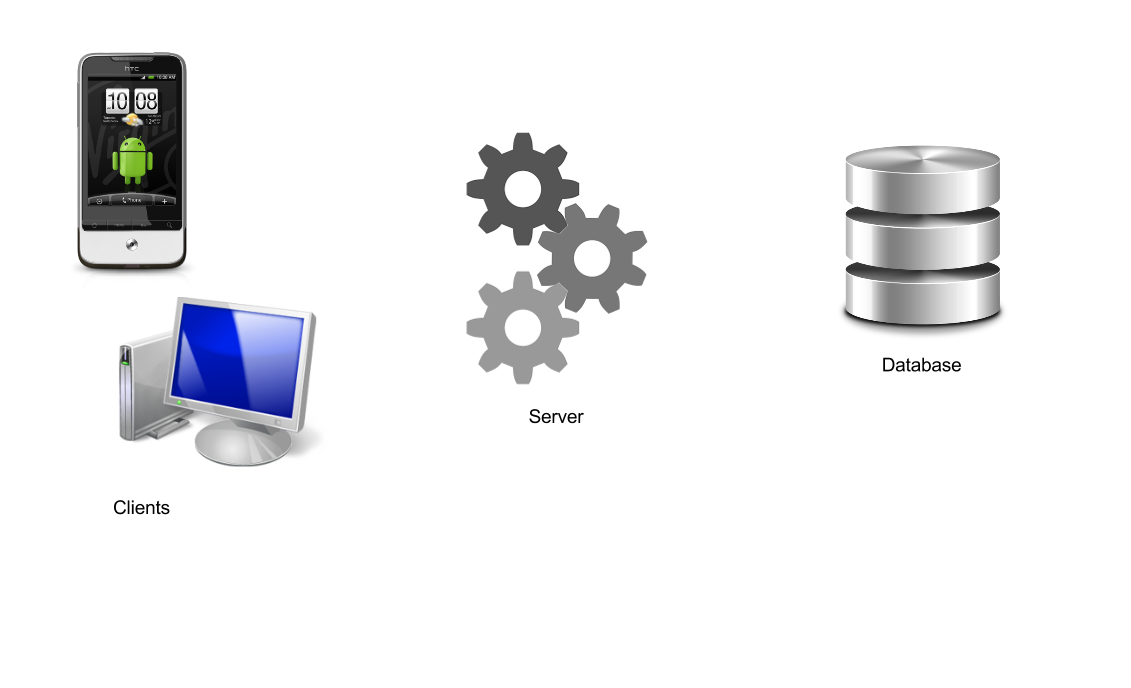
\includegraphics[width=0.8\textwidth]{img/architecture.png}
  \caption{Figure of Architecture}
\end{figure}

Below is a figure that explains the streaming architecture.

\begin{figure}[h]
  \centering
  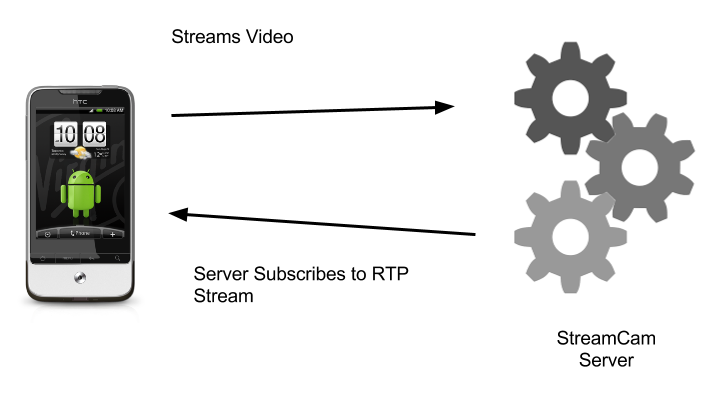
\includegraphics[width=5in]{img/streaming-architecture.png}
  \caption{Figure of Architecture}
\end{figure}

\subsubsection{Major Software Components}
The major software components 
\subsubsection{Major Software Interactions}
\subsubsection{Architectural Design Diagrams}
\subsection{CSC and CSU Descriptions}
\subsubsection{Class Descriptions}
\paragraph{Class Description 1}
\paragraph{Class Description 2}
\paragraph{Class Description n}
\subsubsection{Detailed Interface Descriptions}
\subsubsection{Detailed Data Structure Descriptions}
\subsubsection{Detailed Design Diagrams}
\subsection{Database Design and Description}
\subsubsection{Database Design ER Diagram}
\subsubsection{Database Access}
\subsubsection{Database Security}

%%%%% SDD ENDS HERE
\section{Notes}
\section{Acronyms and Abbreviations}


\end{document}